\begin{mainquestion}{seriesmosbias}{Series PMOS Bias Voltages}

Two identical PMOS transistors $Q_{1}$ and $Q_{2}$ with $k = 1\ \frac{\text{mA}}{V^{2}}$ and $V_{tp} = -\qty{1}{\volt}$ are connected in series as shown in the figure below.

\begin{center}
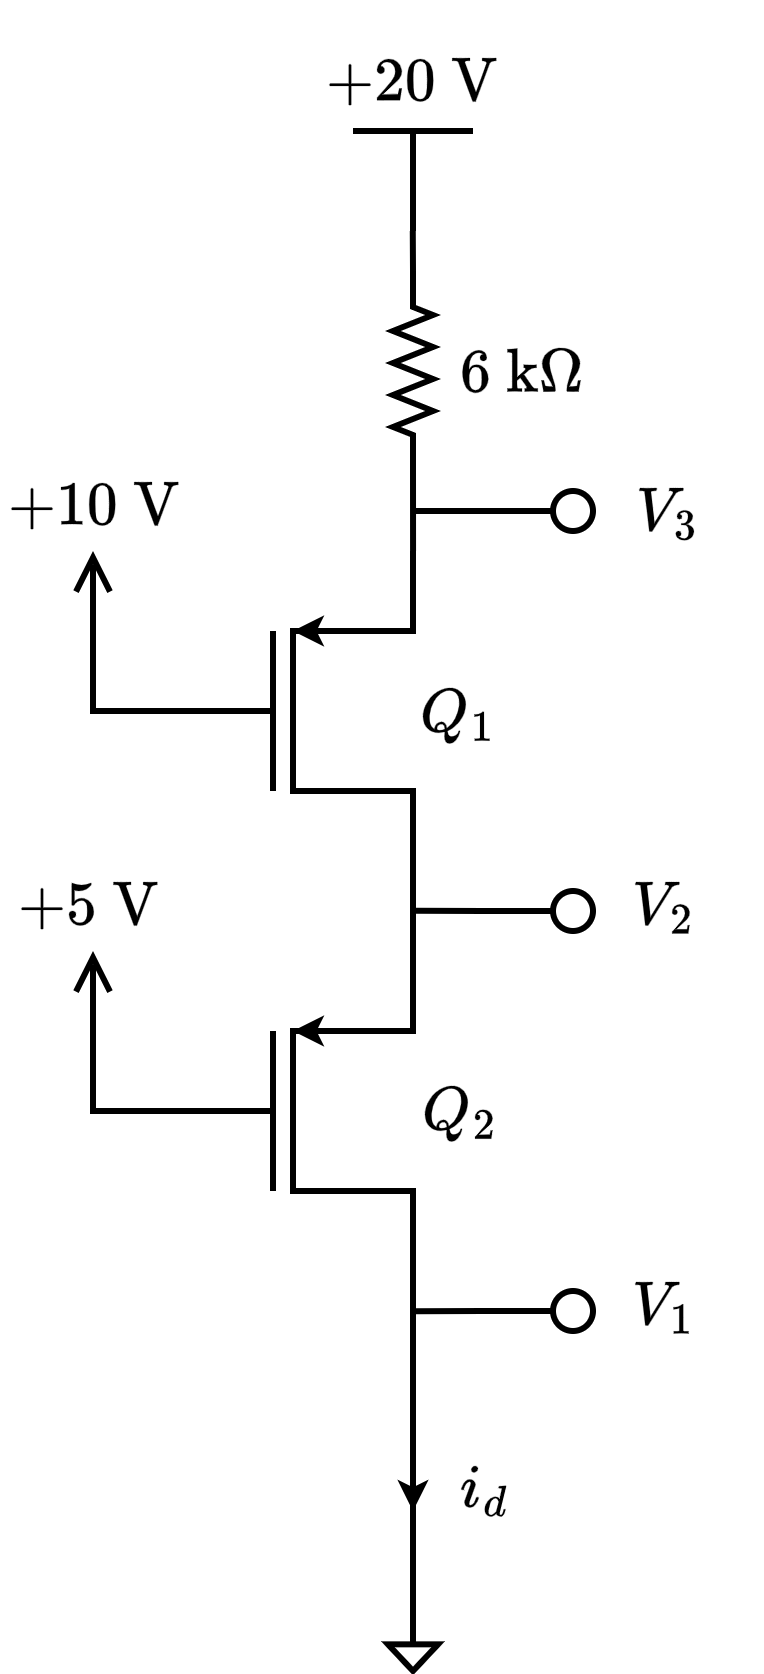
\includegraphics[height=5in]{circuit.png}
\end{center}

\begin{partquestion}{findvoltages}{What are the resulting DC bias voltages $V_{1}$, $V_{2}$, and $V_{3}$?}
\begin{answer}
Well, $V_{1}$ is immediately obvious---it is identically 0 V (ground)! For PMOS saturation:
\begin{align*}
    v_{DS} &\leq v_{GS} - V_{tp} \\
    v_D - v_S &\leq v_G - v_S - V_{tp} \\
    v_D &\leq v_G - V_{tp}
\end{align*}

Consider transistor $Q_{2}$, where $V_{G2} = \qty{5}{\volt}$ and $V_{D2} = \qty{0}{\volt}$. Since $0 \leq 5 - (-1) = 6$, this device will be in saturation as long as it is not in cutoff, which would occur when $v_{SG2} < -V_{tp}$ or equivalently when $V_{2} = v_{S2} < v_{G2} - V_{tp} = 5 - (-1) = \qty{6}{\volt}$. If $Q_{2}$ is in saturation, $Q_{1}$ cannot be in cutoff, or current would not flow through $Q_{2}$. Let us assume that both devices are in saturation and check for possible contradictions that arise with the analysis. Since both transistors have identical $k_{p}$ and $V_{tp}$, and for saturation $i_{D} = \frac{1}{2}k_{p}\left( - V_{GS} + V_{tp} \right)^{2}$, it follows that both must have the same $V_{GS}$ if the currents are the same; that is, $V_{GS1} = V_{GS2}$. So we have the relationship:
\begin{align*}
    5 - V_2 &= 10 - V_3 \\
    V_3 &= 5 + V_2
\end{align*}
Additionally, we have:
\begin{align*}
    i_D &= \frac{1}{2} k_p (-V_{GS1} +V_{tp})^2 \\
    &= \frac{1}{2} k_p (V_{S1} - V_{G1} + V_{tp})^2 \\
    &= \frac{1}{2} (1) (V_3 - 10 - 1)^2 \\
    &= \frac{1}{2} (V_3 - 11)^2
\end{align*}
and
\begin{align*}
    i_D &= \frac{1}{2} k_p (-V_{GS2} +V_{tp})^2 \\
    &= \frac{1}{2} k_p (V_{S2} - V_{G2} + V_{tp})^2 \\
    &= \frac{1}{2} (1) (V_2 - 5 - 1)^2 \\
    &= \frac{1}{2} (V_2 - 6)^2
\end{align*}
so, since this must be equal to the current through the resistor, gives:
\begin{align*}
    \frac{1}{2} (V_2 - 6)^2 &= \frac{20 - V_3}{6} \\
    \frac{1}{2} (V_2 - 6)^2 &= \frac{20 - (5+V_2)}{6} \\
    3 (V_2^2 - 12V_2 +36) &= 15 - V_2 \\
    3V_2^2 - 35V_2 + 93 &= 0
\end{align*}
which has two potential solutions $V_{2} = \qty{4.093}{\volt}$ and $V_{2} = \qty{7.573}{\volt}$. Note the first solution $4.093 < 6$, which we earlier showed is the threshold for $Q_{2}$ to be in saturation, so this solution is invalidated. The second solution $V_{2} = \qty{7.573}{\volt}$ is greater than 6 V, so it leads to a consistent result. It follows directly that $V_{3} = 5 + V_{2} = 5 + 7.573 = \qty{12.573}{\volt}$, which also ensures $Q_{1}$ is in saturation.
\end{answer}
\end{partquestion}

\begin{partquestion}{findcurrent}{At these bias levels, what is the current $i_{D}$?}
\begin{answer}
We can use the equation for current in saturation for either $Q_{1}$ or $Q_{2}$. Let's choose $Q_{1}$:
\begin{align*}
    i_D &= \frac{1}{2} k_p (V_3 - 11)^2 \\
    &= \frac{1}{2} (1) (12.573 - 11)^2 \\
    &= \qty{1.24}{\milli\ampere}
\end{align*}
\end{answer}
\end{partquestion}

\end{mainquestion}
